% Jacob Neumann

% DOCUMENT CLASS AND PACKAGE USE
    \documentclass[aspectratio=169]{beamer}
 
    % Establish the colorlambda boolean, to control whether the lambda is solid color (true), or the same as the picture (false)
    \newif\ifcolorlambda
    \colorlambdafalse % DEFAULT: false
    
    % Use auxcolor for syntax highlighting
    \newif\ifuseaux
    \useauxfalse % DEFAULT: false
   
    % Color settings
    \useauxtrue
    
    \newcommand{\auxColor}{FF4F4F}     % the color of note boxes and stuff
    \newcommand{\presentColor}{FFAB73} % the primary color of the slide borders
    \newcommand{\bgColor}{fff3e6}      % the color of the background of the slide
    \newcommand{\darkBg}{8b98ad}
    \newcommand{\lambdaColor}{\auxColor}
  
    \colorlambdatrue

    \usepackage{comment} % comment blocks
    \usepackage{soul} % strikethrough
    \usepackage{listings} % code
    \usepackage{makecell}

    \setbeamertemplate{itemize items}[circle]
    % \setbeameroption{show notes on second screen=right}

    \usepackage{lectureSlides}
    %%%%%%%%%%%%%%%%%%%%%%%%%%%%%%%%%%%%%%%%%| <----- Don't make the title any longer than this
    \title{Asymptotic Analysis} % TODO
    \subtitle{Awesome slides with an awesome subtitle} % TODO
    \date{01 January 2020} % TODO
    \author{Brandon Wu} % TODO

    \graphicspath{ {./img/} }
    % DONT FORGET TO PUT [fragile] on frames with codeblocks, specs, etc.
        %\begin{frame}[fragile]
        %\begin{codeblock}
        %fun fact 0 = 1
        %  | fact n = n * fact(n-1)
        %\end{codeblock}
        %\end{frame}

    % INCLUDING codefile:
        % 1. In some file under code/NN (where NN is the lecture id num), include:
    %       (* FRAGMENT KK *)
    %           <CONTENT>
    %       (* END KK *)
    
    %    Remember to not put anything on the same line as the FRAGMENT or END comment, as that won't be included. KK here is some (not-zero-padded) integer. Note that you MUST have fragments 0,1,...,KK-1 defined in this manner in order for fragment KK to be properly extracted.
        %  2. On the slide where you want code fragment K
                % \smlFrag[color]{KK}
        %     where 'color' is some color string (defaults to 'white'. Don't use presentColor.
    %  3. If you want to offset the line numbers (e.g. have them start at line 5 instead of 1), use
                % \smlFragOffset[color]{KK}{5}

\begin{document}

% Make it so ./mkWeb works correctly
\ifweb
    \renewcommand{\pause}{}
\fi

\setbeamertemplate{itemize items}[circle]

% SOLID COLOR TITLE (see SETTINGS.sty)
{
\begin{frame}[plain]
    \colorlambdatrue
    \titlepage
\end{frame}
}

\begin{frame}[fragile]
  \frametitle{Lesson Plan}

  \tableofcontents
\end{frame}

\begin{frame}[fragile]
  \frametitle{Last time}

  Last time, we learned about \term{trees}, which are a particular instance of
  \term{datatype declarations}.

  \vspace{\fill}

  We saw how we could represent trees via the \code{Empty} and \code{Node} 
  constructors, as well as how to do proof by structural induction on a tree. 

  \vspace{\fill}

  We then saw how we could use \code{datatype} declarations more generally, to
  define types and values that fit the problem we are trying to solve. We used
  it to define an \code{order} datatype, for comparing two integers.
\end{frame}

\sectionSlide{1}{Asymptotic Complexity}

\begin{frame}[fragile]
  \frametitle{Where we are so far}

  So far, we've been concerned with exploring the expressivity of the Standard ML
  language.

  \vspace{\fill}

  We've learned how we can use fundamental language concepts like 
  \term{pattern matching}, \term{datatype declarations}, and \code{recursion}
  to both state and solve various problems in computer science.

  \vspace{\fill}

  On the first day, functional programming was first explained as a kind of 
  better way of communicating, as programmers. This is not the only thing we
  care about, however! We also care about how well our code performs.
\end{frame}

\begin{frame}[fragile]
  \frametitle{Performance in Computer Science}

  Performance can be difficult to measure, however, because it's not a very
  standardized process! Performance can vary from program to program, of course,
  but also from computer to computer, depending on the hardware.

  \vspace{\fill}

  Even worse is that even on the same computer, performance can vary from run to
  run, due to factors in the computer such as its current CPU load, the amount of 
  power it has, and other low-level factors.

  \vspace{\fill}

  We want to be able to analyze performance mathematically, in a way that is 
  agnostic to these silly details.
\end{frame}

\begin{frame}[fragile]
  \frametitle{Big-O Notation}

  We also observe that as time goes on, the amount of data that computers are
  asked to deal with has gone up significantly. Gone are the days of punching
  data into cards, now we store petabytes of data in the cloud.

  \vspace{\fill}

  As such, we want to measure performance in a way agnostic to silly hardware
  details, but still sensitive to mathematical differences in how an algorithm
  runs.

  \vspace{\fill}

  \defBox{}{\, We use \term{Big-O notation} to describe the behavior of a 
  function, in the limit of the size of its input. This function usually
  denotes the computational cost of a program.}
\end{frame}

\begin{frame}[fragile]
  \frametitle{Big-O, Formally}

  Formally, we take a function $f : \mathbb{N}^+ \to \mathbb{N}^+$, which in
  our case describes the abstract cost of running some program. 

  \vspace{\fill}
  
  The input is some metric of the data input (the length of a list, the 
  size of a number) and the output is the number of abstract units that it 
  costs to run on that input.

  \vspace{\fill}

  For another function $g : \mathbb{N}^+ \to \mathbb{N}^+$, we say that
  $f \in O(g)$ if there exists $n_0, c > 0$ such that, for all $n \geq n_0$,
  $f(n) \leq cg(n)$.
\end{frame}

\begin{frame}[fragile]
  \frametitle{I Don't Speak Math}

  OK, that's a lot to digest. What does it really mean?

  \vspace{\fill}

  All this is describing is that a function
  $f$ (the run-time function) is in $O(g)$, such as $O(n^2)$ or $O(n)$ (the 
  complexity class), if there exists an an input size $n_0$, beyond with the
  run-time function is always less than the complexity class function (scaled by
  a constant factor).

  \vspace{\fill}

  We need the constant factor for cases such as $f(n) = 2n$ and $g(n) = n$, where
  there is no value such that $f(n) \leq g(n)$. Despite that, however, the former
  function is still a linear function, so we should be able to scale $g$
  by a constant factor (say, $2.5$) and conclude $f \in O(g)$. 
\end{frame}

\begin{frame}[fragile]
  \frametitle{I Don't Speak Math}

  This is why $n$ and $n_0$ are important:
  \vspace{\fill}
  \centerline{
  \begin{minipage}{0.4\textwidth}
    \includegraphics[scale=0.4]{graph1} \\ 
    $f$ is always less than $g$.
  \end{minipage}
  \begin{minipage}{0.4\textwidth}
    \includegraphics[scale=0.4]{graph2}
    $f$ is not always less than $g$
  \end{minipage}
  }
\end{frame}

\begin{frame}[fragile]
  \frametitle{I Don't Speak Math}

  This is why $c$ is important:
  \vspace{\fill}
  \centerline{
  \begin{minipage}{0.4\textwidth}
    \includegraphics[scale=0.4]{graph4}
    $f$ is greater than $g$
  \end{minipage}
  \begin{minipage}{0.4\textwidth}
    \includegraphics[scale=0.4]{graph3}
    but not when $g$ is scaled by 3
  \end{minipage}
  }

\end{frame}

\begin{frame}[fragile]
  \frametitle{The Asymptotic Hierarchy}

  In general, in this class, time complexity will fall into a few common buckets,
  and not really venture outside of them.
  
  \vspace{\fill}

  It is important to know how these complexity classes are related!

  $$O(1) < O(\log n) < O(n) < O(n \log n) < O(n^2) < O(n^3) < ...$$

  \vspace{\fill}

  In general, we will only see complexity up until $O(n^2)$.

  \vspace{\fill}

  It is worth noting that the $\in$ relation for asymptotic complexity is more
  permissive than we need! If we have $f \in O(n)$, then it is also true that 
  $f \in O(n \log n)$, and $f \in O(n^2)$, and so on.

  \vspace{\fill}

  We want to find the \textit{least} complexity class that captures this relation.
  This is called a \textit{tight asymptotic bound}.
\end{frame}

\begin{frame}[fragile]
  \frametitle{Asymptotic Complexity at a Glance}

  Here are some examples of common operations that fall into these buckets:

  \vspace{\fill}

  \begin{itemize}
    \item $O(1)$ - Consing an element onto a list, multiplying two numbers, 
    stepping an expression once
    \item $O(\log n)$ - Binary searching an interval $n$ wide, finding an
    element in a binary search tree
    \item $O(n)$ - Computing the length of a list, finding the last element 
    of a list, summing the nodes of a tree 
    \item $O(n \log n)$ - Mergesort and quicksort
    \item $O(n^2)$ - Insertion sort, selection sort
  \end{itemize}

\end{frame}

\begin{frame}[fragile]
  \frametitle{Implicit Functions}

  Note that, when computing asymptotic complexity, there is always an underlying
  function $f$ that we are approximating the behavior of. This function always
  takes in some number that denotes the "size of the input".

  \vspace{\fill}

  In the case of numbers, this is just the number itself.

  \vspace{\fill}

  In the case of something like "computing the length of the list", this is the
  length of the list. In the case of trees, this could be the number of nodes in
  the tree.
  
  \vspace{\fill}

  It's important to realize that, although we are being casual and not specifying
  things explicitly, these underlying size metric are still there!
\end{frame}

\sectionSlide{2}{Work and Recurrences}

\begin{frame}[fragile]
  \frametitle{Applied Big-O}

  Big-O notation is useful conceptually, but not very useful if we can't reliably
  come to define the function $f$ that we would like to find the bound of!

  \vspace{\fill}

  Casually, we might skip the function $f$ and just go straight to the bound, by
  estimating the amount of times that work is done. For instance, for the following
  function:

  \vspace{5pt}

  \begin{codeblock}
    fun length ([] : int list) : int = 0
      | length (x::xs) = 1 + length xs
  \end{codeblock}

  \vspace{5pt}

  without even thinking, we might say that it is $O(n)$, because we iterate over
  the entire list.

  \vspace{\fill}

  This is an informal way of thinking, however! One of the strengths of functional
  programming is that we will be able to give this analysis a more rigorous
  treatment.
\end{frame}

\begin{frame}[fragile]
  \frametitle{Recurrences}

  To do this, we will specify a \term{recurrence relation} for each function that
  we wish to analyze.

  \vspace{\fill}
  
  \defBox{}{\, A \term{recurrence relation} is a series of mathematical equations
  that specifies the run-time cost of a recursive function, defined in terms of
  itself.}

  \vspace{\fill}

  We then solve the recurrence relation to obtain a function that describes the
  \term{work} of the function, in some size metric, and then place it in a 
  complexity class.

  \vspace{\fill}

  \defBox{}{\, The \term{work} of a function is its run-time cost.}
\end{frame}

\begin{frame}[fragile]
  \frametitle{Formulating the Recurrence}

  Let's take the \code{fact} function, as a starter. 

  \vspace{\fill}

  \begin{codeblock}
    fun fact (0 : int) : int = 1
      | fact n = n * fact (n - 1)
  \end{codeblock}

  \vspace{\fill}

  We obtain the recurrence by analyzing the work done in each case. We obtain
  two equations, for the two cases of the function:

  \vspace{\fill}

  $$W_{\code{fact}}(0)\footnotemark = c_0$$
  $$W_{\code{fact}}(n) = c_1 * W_{\code{fact}}(n - 1)$$

  \footnotetext[1]{$W_{\code{fact}}(0)$, for "work of \code{fact} on input size 0"}
\end{frame}

\begin{frame}[fragile]
  \frametitle{Understanding the Recurrence}

  $$W_{\code{fact}}(0) = c_0$$
  $$W_{\code{fact}}(n) = W_{\code{fact}}(n - 1) + c_1$$

  \vspace{\fill}

  In the first case, we return an unspecified constant $c_0$. Work is measured
  in arbitrary abstract units, and we don't necessarily know how many of those 
  are taken up by returning $1$. It's nonzero, because there is some
  amount of work that needs to be done, but it's otherwise unknown, so we use a 
  placeholder constant $c_0$. 

  \vspace{\fill}

  In the second case, we do some constant amount of work, again. It's not necessarily
  the exact same as the previous case, so we just call it $c_1$. We also do the work
  of computing \code{fact} on an input that is 1 smaller.
\end{frame}

\begin{frame}[fragile]
  \frametitle{Solving the Recurrence}

  Now that we have the recurrence, we can go ahead and try to solve. We will
  use a technique called \term{unrolling}.

  \vspace{\fill}

  \defBox{}{\, The \term{unrolling} method for solving recurrences entails
  just expanding the definition of the recurrence, finding a pattern,
  and then writing a closed form.}

  \vspace{\fill}

  So we obtain, when $n$ is the size of the number \code{n} in the expression \code{fact n}:
  \begin{align*}
    W_{\code{fact}}(n) &= W_{\code{fact}}(n - 1) + c_1 \\
                       &= W_{\code{fact}}(n - 2) + c_1 + c_1 \\ 
                       &= ...  \\ 
                       &= \sum_{i = 0}^{n} c_1 + c_0 \\
                       &= n \cdot c_1 + c_0
  \end{align*}
\end{frame}

\begin{frame}[fragile]
  \frametitle{Note on Formality}

  When using the unrolling method, we're not being super strict, but the
  idea is just to demonstrate that you know that there is a pattern, and
  that the recurrence definitely will expand to the given closed form!

  \vspace{\fill}

  We are not going to be super picky, but it matters that we can follow
  along with your reasoning.
\end{frame}

\begin{frame}[fragile]
  \frametitle{Solving the Recurrence}

  Finally, once we have a closed form, this is essentially our function $f$.
  We now want to find a complexity class for it.

  \vspace{\fill}

  If you followed all the steps correctly, it should be fairly obvious what
  is a tight bound for it. For instance, for the closed form

  \vspace{\fill}

  $$W_{\code{fact}}(n) = n \cdot c_1 + c_0$$

  \vspace{\fill}

  we can clearly tell that it is in $O(n)$, because it is a linear function in
  $n$.
\end{frame}

\begin{frame}[fragile]
  \frametitle{A Worst-Case Example}

  Consider the following artificial SML function:

  \begin{codeblock}
    fun findFirstEven ([] : int list) : int option = NONE
      | findFirstEven (x::xs) =
          if x mod 2 = 0 then
            SOME x
          else
            findEven xs 
  \end{codeblock}

  This function, \code{findFirstEven}, seeks to find the first even number in an SML
  list of integers. Since there might not be such a number, it returns an optional
  value.

  How might we write a recurrence for this function?
\end{frame}

\begin{frame}[fragile]
  \frametitle{A Worst-Case Recurrence}

  First, we need to identify the parameter for our recurrence. What number is our recurrence
  measured in terms of?

  For lists, we'll choose to pick the length of the list. It's the most obvious metric.

  For the base case, it's fairly simple. We do a constant amount of work, so we produce:

  $$W_{\code{findFirstEven}}(0) = c_0$$

  What about the recursive case? Well, the recursive case is actually \textit{two} cases.
\end{frame}

\begin{frame}[fragile]
  \frametitle{A Worst-Case Recurrence}

  Asymptotic complexity is measured in terms of \term{worst-case behavior}.

  This means that, across the entire range of inputs that the function could be given, we are interested
  in measuring the complexity when the function is given an input that causes the \textit{most work for it to do}.

  While \code{findFirstEven}, in the recursive case, \textit{could} terminate immediately upon looking at the first
  number, to be truly pessimistic we will assume that there is no such even number in the list, which will cause us
  to always enter back into the recursive case.

  When $n$ is the length of \code{L} in the expression \code{findFirstEven L}: 
  $$W_{\code{findFirstEven}}(n) = W_{\code{findFirstEven}}(n - 1) + c_1$$
  because we call the function again on a list of length one smaller, and do a constant amount of work.
\end{frame}

\begin{frame}[fragile]
  \frametitle{The Recurrence Formula}

  Now that we've done a few examples, we're ready to identify the general formula for 
  analyzing the asymptotic complexity of a function:

  Given an SML function \code{f} that we seek to find the complexity of, we should:

  \begin{itemize}
    \item Identify the size parameter, $n$, that the recurrence is in terms of. This could be something like
    the length of a list, the size of the number, etc.
    \item Write a recurrence for the function. This entails writing an equation for every case it takes, in the
    \textit{worst case}. 
    \item Simplify the recurrence into a closed form in $n$. 
    \item Estimate a complexity class from the recurrence
  \end{itemize}
\end{frame}

\begin{frame}[fragile]
  \frametitle{A Blast from the Past}

  Remember the \code{rev} function?

  \begin{codeblock}
    fun rev ([] : int list) : int list = []
      | rev (x::xs) = rev xs @ [x]
  \end{codeblock}

  Well, this is them now:

  \begin{codeblock}
    fun trev ([] : int list, acc : int list) = acc
      | trev (x::xs, acc) = trev (xs, x::acc)

    fun rev (L : int list) : int list = trev (L, [])
  \end{codeblock}

  We said that our original implementation of \code{rev} was undesirable because it wasn't tail recursive.

  Not only does that matter for how much space it takes, but how much time as well! Let's write the recurrence.
\end{frame}

\begin{frame}[fragile]
  \frametitle{A Blast from the Past}

  \begin{codeblock}
    fun @ ([] : int list, ys : int list) : int list = ys
      | @ (x::xs, ys) = x :: (xs @ ys) 

    fun rev ([] : int list) : int list = []
      | rev (x::xs) = rev xs @ [x]
  \end{codeblock}

  We need to first write a recurrence for \code{@}, before we can tackle \code{rev}.
\end{frame}

\begin{frame}[fragile]
  \frametitle{Don't \code{@} Me}

  \begin{codeblock}
    fun @ ([] : int list, ys : int list) : int list = ys
      | @ (x::xs, ys) = x :: (xs @ ys) 
  \end{codeblock}

  But, how should we write a recurrence for \code{@}? It has two arguments! Our recurrences only take in
  a single size parameter.

  We will just identify a single parameter that it makes sense to measure the size of the input in. We mentioned
  before that \code{@} only ever looks at the left list, so we'll only measure our work in terms of the length of
  the left list.

  Where $n$ is the length of \code{L}, when calling \code{L @ R}:
  $$W_{\code{@}}(0) = c_0$$
  $$W_{\code{@}}(n) = W_{\code{@}}(n) + c_1$$  

  We can write out the work as before, but we know that this will go to the closed form
  $$n \cdot c_1 + c_0$$
  which is in $O(n)$.
\end{frame}

\begin{frame}[fragile]
  \frametitle{Onto \code{rev}}

  Now we write the recurrence for \code{rev}:
  \begin{codeblock}
    fun rev ([] : int list) : int list = []
      | rev (x::xs) = rev xs @ [x]
  \end{codeblock}

  Where $n$ is the length of \code{L}, in the expression \code{rev L}:
  $$W_{\code{rev}}(0) = c_0$$
  $$W_{\code{rev}}(n) = W_{\code{rev}}(n - 1) + ???$$

  We make a call to \code{rev}, which has work $W_{\code{rev}}(n - 1)$. But what about after? We call
  \code{@}, but how big is the length of the list?

  Fortunately, we know that the length of \code{rev xs} is the same as the length of \code{xs}, so we can write:
  $$W_{\code{rev}}(n) = W_{\code{rev}}(n - 1) + W_{\code{@}}(n - 1) + c_1\footnotemark$$

  \footnotetext[2]{Don't forget this $c_1$. There is still a constant amount of work being done here.}
\end{frame}

\begin{frame}[fragile]
  \frametitle{Solving \code{rev}}

  $$W_{\code{rev}}(0) = c_0$$
  $$W_{\code{rev}}(n) = W_{\code{rev}}(n - 1) + W_{\code{@}}(n - 1) + c_1\footnotemark$$

  Now to solve the recurrence, we get:

  \begin{align*}
    &= W_{\code{rev}}(n)
    &= W_{\code{rev}}(n - 1) + W_{\code{@}}(n - 1) + c_1
    &= W_{\code{rev}}(n - 1) + c_2 \cdot (n - 1) + c_1
    &= W_{\code{rev}}(n - 2) + W_{\code{@}}(n - 2) + c_1 + c_2 \cdot (n - 1) + c_1
    &= W_{\code{rev}}(n - 2) + c_2 \cdot (n - 2) + c_1 + c_2 \cdot (n - 1) + c_1
  \end{align*}
\end{frame}

\begin{frame}[fragile]
  \frametitle{Solving \code{rev}}

  \begin{align*}
    &= W_{\code{rev}}(n - 2) + c_2 \cdot (n - 2) + c_1 + c_2 \cdot (n - 1) + c_1
    &= ...
    &= \sum_{i = 0}^n c_2 \cdot (n - i) + n \cdot c_1 + c_0 
  \end{align*}

  The first term follows from adding a $c_2 \cdot (n - i)$ at the $i$th step of the expansion.

  The second follows from adding a $c_1$ per step of the expansion.

  The final term comes from the base case.

  We apply a handy math fact, which is that $\sum_{i = 0}^n (n - i) = \sum_{i = 0}^n i = 1 + 2 + ... + n = \frac{n(n + 1)}{2}$,
  which is upper bounded by $n^2$.

  So ultimately, we obtain
  $$= O(n^2) \cdot c_2 + n \cdot c_1 + c_0 \in O(n^2)$$

  \code{rev} is quadratic time, which is really bad!
\end{frame}

\begin{frame}[fragile]
  \frametitle{A \code{rev}-trospection}

  In hindsight, we could have predicted this. The recursive case of \code{rev} essentially appends the prefix of the list 
  over and over again, recursively. 

  But with a recurrence, we now have a mathematical justification for our asymptotic analysis. We know for sure that the 
  \code{rev} function is quadratic time. What will we do about it?

  Well, let's analyze \code{trev}. How much better does it do?
\end{frame}

\begin{frame}[fragile]
  \frametitle{A \code{trev}-elevation}

  \begin{codeblock}
    fun trev ([] : int list, acc : int list) = acc
      | trev (x::xs, acc) = trev (xs, x::acc)
  \end{codeblock}

  To analyze \code{trev}, we note that the right list is never touched, so we will again measure in terms of the
  length of the first list.

  Where $n$ is the length of \code{L} in the expression \code{trev (L, acc)}:
  $$W_{\code{trev}}(0) = c_0$$
  $$W_{\code{trev}}(n) = W_{\code{trev}}(n - 1) + c_1$$

  We know what this solves to. We get a happy bound of $O(n)$.
\end{frame}

\begin{frame}[fragile]
  \frametitle{Some Takeaways}

  We just demonstrated how we can use math and \term{recurrences} to formally reason about the run-time of 
  functional programs.
  
  This came out of the fact that due to \code{purity}, functions always behave the same on the same arguments.
  We can define our \code{W} function and know that it is truly a \textit{function}, and returns the same results
  on the same inputs.

  In addition, due to the recursive nature of the functions we wrote, the recurrences came naturally. It only took
  two cases to specify the run-time of the function, for most of our analyses, and solving it was just math.

  Functional programs help us reason about our code!
\end{frame}

\sectionSlide{2}{Parallelism and Span}

\begin{frame}[fragile]
  \frametitle{My Heart is in the Work}

  Earlier this lecture, we explored the idea of \term{work}, which is the run-time cost of a particular function,
  varied over the size of its input. We saw that we could measure work in terms of \textit{abstract units}, related 
  to the number of steps that we took to evaluate an expression, in our model of SML. For instance:

  \code{(1 + 2) + (3 + 4)} $\stepsTo$ \code{3 + (3 + 4)} $\stepsTo$ \code{3 + 7} $\stepsTo$ \code{10} 

  We know that each of these steps takes some constant number of work, so in abstract units we would say it has constant work. 

  But this isn't quite true in the real world.
\end{frame}

\begin{frame}[fragile]
  \frametitle{Real World Computation}

  Let's have a race! 

  In lecture, we're going to have one person count the number of people in the room.

  Then, we're going to have a team of three people count the people in the room.

  Let's see who wins.
\end{frame}

\begin{frame}[fragile]
  \frametitle{Real World Parallelism}

  Counting is a problem that can make use of \term{parallelism}.

  \defBox{\, \term{Parallelism} is when a process is able to execute some of its tasks at the
  same time.}

  Usually, this happens at the hardware level on a multicore machine, by the processor being
  able to delegate distinct instructions to be performed on different "cores", which can
  communicate answers with each other. 
  
  We will safely ignore most of that, and just assume that multicore machines exist, though.
  
  It's hard to pick a number for how many, however. So let's just assume we have infinitely many.
\end{frame}

\begin{frame}[fragile]
  \frametitle{To Infinity...}

  Having infinite cores sounds like a superpower that should elevate us to computational deities.
  Infinite cores? Infinite power!

  It's not quite the case, though.

  Consider the problem of making a sandwich.
\end{frame}

\begin{frame}[fragile]
  \frametitle{ Sandwich Complexity }

  If there were an infinite amount of me, I might want infinitely many sandwiches.

  But, I can't just instantly make a sandwich, even if I had more hands available. I have to toast the bread,
  which means I need to wait for the pan to heat up, and I can't toast the bread, because I need to slice it from the
  loaf, and I can't slice it from the loaf, because there's only two sides and maybe another version of me wants to
  slice it first. 

  \noteBox{}{\, Making a sandwich is hard.}

  This is the notion of \term{task dependency} in parallel computing.

  \defBox{}{\, When computing in parallel, some tasks have \term{dependencies}, meaning they cannot be completed until
  other tasks are finished.}
\end{frame}

  
\begin{frame}[fragile]
  \frametitle{ Sandwich Dependency Graph }

  \makebox[\textwidth][c]{
    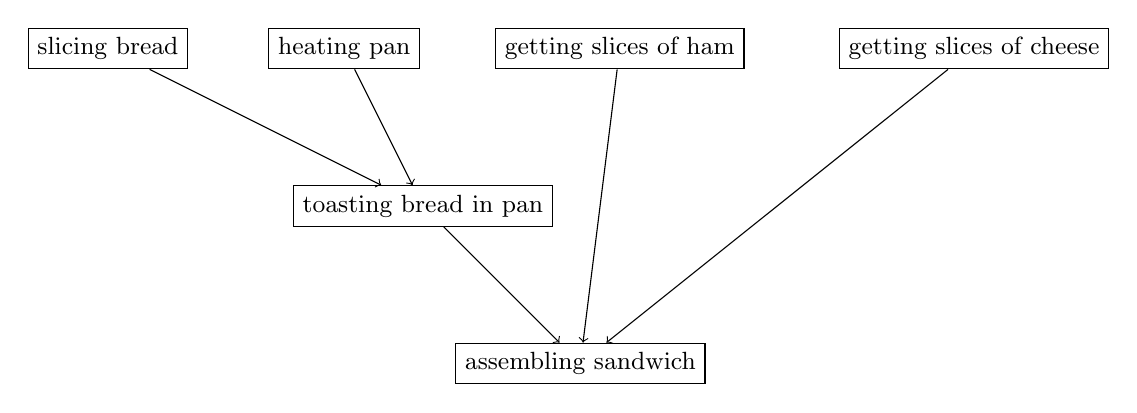
\begin{tikzpicture}
      \node[shape=rectangle,draw=black] (A) at (-4,4) {\small slicing bread};
      \node[shape=rectangle,draw=black] (B) at (-1,4) {\small heating pan};
      \node[shape=rectangle,draw=black] (D) at (2.5,4) {\small getting slices of ham};
      \node[shape=rectangle,draw=black] (E) at (7,4) {\small getting slices of cheese};

      \node[shape=rectangle,draw=black] (C) at (0,2) {\small toasting bread in pan};
      \node[shape=rectangle,draw=black] (F) at (2,0) {\small assembling sandwich} ;

      \draw[->] (A) -- (C);
      \draw[->] (B) -- (C);
      \draw[->] (C) -- (F);
      \draw[->] (D) -- (F);
      \draw[->] (E) -- (F);
  \end{tikzpicture}
  }

  Question: \textbf{How long does it take to make a sandwich?}
  Answer: \textbf{The length of the longest path.}
\end{frame}

\begin{frame}[fragile]
  \frametitle{ Task Dependency Graph }

  This demonstrates the notion of a \term{task dependency graph}.

  \defBox{}{\, A \term{task dependency graph} is an acyclic graph which shows the relationship between
  tasks and their dependencies. The nodes are tasks, annotated with time to complete, and the edges
  go from tasks that are preconditions to other tasks.}

  In a task dependency graph, with only a single processor, we cannot avoid having to visit every single
  node. It doesn't really matter what order we do it in, but we have to pay cost equal to the sum of all
  the nodes.

  With infinitely many processors, because we can start unrelated tasks at the same time, the amount of time
  spent is just the length of the \textit{longest} dependency chain in the graph. In essence, the height
  of the graph.
\end{frame}

\begin{frame}[fragile]
  \frametitle{ Circling Back Around }

  In terms of concrete vocabulary, this demonstrates the difference between \term{work} and \term{span}.

  \defBox{}{\, We say that the \code{work} of a process is the time expended using a single processor. }

  \defBox{}{\, We say that the \code{span} of a process is the time expended using infinitely many processors. }

  We said earlier that in SML, tuples are evaluated left to right. In a world with infinitely many processors, we 
  will assume that elements of a tuple can be computed \textit{at the same time}.

  We wrote recurrences labeled with $W$ earlier -- $W$, for \textit{work}. Now, we will write recurrences for \textit{span}.
\end{frame}

\begin{frame}[fragile]
  \frametitle{ A Span Recurrence } 

  Let's compute the span of the \code{length} function. The process will look very similar, but we will assume that any
  tuples are evaluated in parallel. 

  \begin{codeblock}
    fun length ([] : int list) : int = 0
      | length (x::xs) = 1 + length xs
  \end{codeblock}

  Where $n$ is the length of the list \code{L} in the expression \code{length L}:
  $$S_{\code{length}}(0) = c_0$$
  $$S_{\code{length}}(n) = \max(c_1, S_{\code{length}}(n - 1)) + c_2$$ 

  Then we have:
  \begin{align*}
    S_{\code{length}}(n) \\ 
    &= \max(c_1, S_{\code{length}}(n - 1)) + c_2 \\
    &= S_{\code{length}}(n - 1) + c_2
    &= ...
    &= O(n)
  \end{align*}
\end{frame}

\begin{frame}[fragile]
  \frametitle{ A \code{span}-ner In The \code{work}s }

  What gives? We got the same bound, even though we had infinitely many processors!

  This is because lists are inherently a sequential structure. Even if you had many 
  processors, you can't touch the second list element until you look at the first.
  In essence, every list has a single "child", if we view \code{xs} as the child to
  \code{x::xs}.

  What's a data structure that has more than one child?
\end{frame}

\begin{frame}[fragile]
  \frametitle{ Span and Trees }

  Let's analyze the span of a function on trees! 

  \begin{codeblock}
    fun treesum (Empty : tree) : int = 0
      | treesum (Node (L, x, R)) = treesum L + x + treesum R
  \end{codeblock}

  We need a metric for the size of the tree, though. There's actually two options -- 
  the number of nodes in the tree, or the height of the tree.
\end{frame}

\begin{frame}[fragile]
  \frametitle{ Tree Recurrence: Nodes }

  Both are valid ways to go about it. Let's try it first by using $n$, the 
  number of nodes in the tree.

  \begin{codeblock}
    fun treesum (Empty : tree) : int = 0
      | treesum (Node (L, x, R)) = treesum L + x + treesum R
  \end{codeblock}

  Where $n$ is the number of nodes in \code{T}, in the expression \code{treesum T}:

  $$S_{\code{treesum}}(0) = c_0$$
  $$S_{\code{treesum}}(n) = ???$$

  What should we put for the recursive case? Because of infinite processors,
  we can consider the calls to \code{treesum L} and  \code{treesum R} to all be 
  executed in parallel. But what is the number of nodes in each?
\end{frame}

\begin{frame}[fragile]
  \frametitle{ Tree Recurrence: Unbalanced Tree }

  For an arbitrary tree, we can't possibly know the number of nodes in the
  left and right tree. This is where worst-case analysis will save us.

  To simplify our analysis, we will simply pick the configuration that is the
  worst for us. The worst case for \code{treesum} is when the input tree is
  a "spine", or a straight line. Thus, we will assume the number of nodes in the
  left is $n - 1$, and in the right, $0$.

  So we obtain:
  $$S_{\code{treesum}}(n) = \max(S_{\code{treesum}}(n - 1), + S_{\code{treesum}}(0)) + c_1$$
  $$S_{\code{treesum}}(n) = S_{\code{treesum}}(n - 1) + c_1$$

  where the constant work is again, the residual work of addition and retrieving the
  other results.
\end{frame}

\begin{frame}[fragile]
  \frametitle{ Tree Recurrence: Unbalanced Tree }

  $$S_{\code{treesum}}(0) = c_0$$
  $$S_{\code{treesum}}(n) = S_{\code{treesum}}(n - 1) + c_1$$
  
  Wait a second, we've seen this before. If we swap the $S$ for $W$, this is the same
  recurrence as we've been getting the whole time!

  We know this is in $O(n)$.
\end{frame}

\begin{frame}[fragile]
  \frametitle{ Unbalanced Is Overpowered }

  We see that our span bound on an unbalanced tree is still $O(n)$! Even with
  infinite processors, we can't do better than linear complexity.

  This kind of makes sense, because a tree that is just a single line is basically 
  a list with extra metadata. \code{treesum} isn't doing much more than
  \code{length}, so we get a similar span bound!

  What if we assume that the tree is balanced?
\end{frame}

\begin{frame}[fragile]
  \frametitle{ Tree Recurrence: Balanced Tree }

  The base case is as before.

  In this case, we can assume that each call to \code{treesum} is on a tree
  with roughly half the nodes as the input. For simplicity, let's assume we
  have a tree with $n = 2^k$, for some $k$. 

  Then, we get:
  $$S_{\code{treesum}}(n) = \max(S_{\code{treesum}}(\frac{n}{2}), S_{\code{treesum}}(\frac{n}{2})) + c_1$$
  $$S_{\code{treesum}}(n) = S_{\code{treesum}}(\frac{n}{2}) + c_1$$
\end{frame}

\begin{frame}[fragile]
  \frametitle{ Tree Recurrence: Balanced Tree }

  \begin{align*}
    &= S_{\code{treesum}}(n) \\ 
    &= S_{\code{treesum}}(\frac{n}{2}) + c_1 \\
    &= S_{\code{treesum}}(\frac{n}{4}) + c_1 + c_1 \\
    &= S_{\code{treesum}}(\frac{n}{8}) + c_1 + c_1 \\
    &= ... \\
    &= \log n \cdot c_1
  \end{align*}

  because the number of times we can divide $n$ by $2$ is exactly the
  logarithm of $n$, base 2.

  So this is in $O(\log n)$.
\end{frame}

\begin{frame}[fragile]
  \frametitle{ The Power of Span }

  Finally, we obtain a better bound! On balanced trees, we can parallelize
  more work, so we are able to run \code{treesum} in only log time, as opposed
  to linear. That's a big difference!
  
  We will see that parallelism is a powerful tool that will help us achieve
  better bounds in a variety of situations. This is only the tip of the
  iceberg.  
\end{frame}

\begin{frame}[fragile]
  \frametitle{ A Note on Realism }

  One point that needs to be said before the end of lecture: yes, having
  infinite processors is impossible\footnotemark.

  This doesn't cheapen the findings we discussed. We're dealing with 
  mathematical abstractions, and being able to assume as many processors
  as needed is one of them.

  In reality, performance is somewhere between the work and the span, but
  the span remains a useful mathematical ideal. Brent's Theorem says more
  on the matter:

  brent's theorem
  \footnotetext[1]{I knew this the whole time!!!!}
\end{frame}

\begin{frame}[plain]
	\begin{center} Thank you! \end{center}
\end{frame}


\end{document}

